\section{Zielsetzung}
\label{sec:Zielsetzung}

In diesem Versuch soll die Brennweite $f$ auf unterschiedliche Arten von verschiedenen Linsen beziehungsweise Linsensystem bestimmt werden. Als erstes sollen das Abbildunggesetz und die Linsengleichung verifiziert werden. Die jeweiligen Brennweiten sollen nach der Methode von Abbe und Bessel untersucht und bestimmt werden. 

\section{Theorie}
\label{sec:Theorie}

Die Linsen bestehen aus einem durchsichtigem Material, welches opticher dichter ist als "Luft". Wenn Licht auf eine Linse trifft, wird es nach dem Brechungsgesetz gebrochen. Es gibt viele Formen von Linsen und Linsenarten, die Licht auf unterschiedlichste Art brechen. Die bekanntesten Linsenformen sind Sammellinsen und Zerstreuungslinsen.
\begin{figure}[h!]
	\centering
	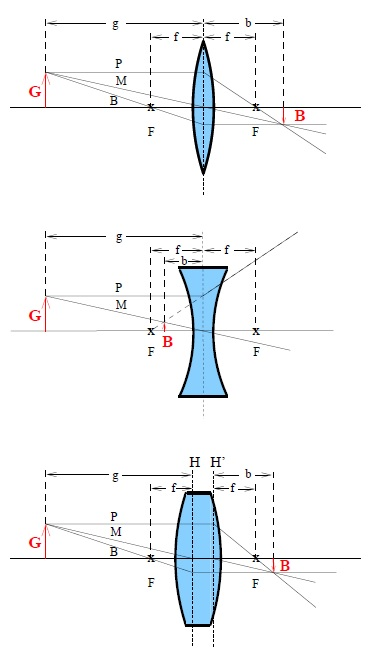
\includegraphics[width=0.5\linewidth]{../../GeometrischeOptik}
	\caption{Konstruktionsstrahlen bei den verschiedenen Linsentypen, \cite[1]{anleitung408}.}
	\label{fig:geometrischeoptik}
\end{figure}
Diese sind in der Abbildung \ref{fig:geometrischeoptik} zu sehen. Eine Sammellinse ist am Rand etwas dünner als in der Mitte und diese sind dadurch charakterisiert, dass sie ein parallel einfallendes paralleles Lichtbündel nach dem Durchlaufen der Linse in einem Punkt sammeln, dem Brennpunkt (s. Abbildung \ref{fig:geometrischeoptik} oben). Bei den Sammellinsen sind die Brennweite $f$ und die Bildweite $b$ positiv, sodass es ein reelles Bild entstehen kann. 

Im Gegensatz zu den Sammellinsen, sind die Brennweite $f$ und die Bildweite $b$ negativ bei einer Zerstreuungslinse, so dass es ein virtuelles Bild entstehen kann (s. Abbildung \ref{fig:geometrischeoptik} in der Mitte). Diese sind auch in der Mitte etwas dünner als am Rand.

In der Abbildung \ref{fig:geometrischeoptik} ist unten noch eine dicke Sammellinse zu sehen. Das Modell bei einer dünnen Linse ist es so konzipiert,  dass die Brechung auf die Mittelebene reduziert wird. Dies funktioniert nur für die dünnen Linsen, denn bei den dicken werden zwei zusätzlichen Hauptebenen hinzugefügt, wo die Strahlen gebrochen sein müssen.

Wichtig für die Zusammenstellung einer Linse sind die folgenden drei ausgezeichneten Strahlen aus der Abbildung \ref{fig:geometrischeoptik}: 

$\bullet$ der Parallelstrahl P verläuft parallel zur optischen Achse zur Linse und trifft auf der anderen Seite der Linse, sodass er zum Brennpunkt wird;

$\bullet$ der Mittelpunktstrahl M läuft durch das Linsenzentrum und bleibt ungebrochen, also er wird nicht abgelenkt;

$\bullet$ der Brennpunktstrahl B wird zum Parallelstrahl, da er zuerst durch den Brennpunkt läuft und auf der anderen Seite der Linse parallel zur optischen Achse verläuft.

Mit den Strahlensätzen und Zusammenstellung einer Linse lässt sich das Abbildungsgesetz formulieren:
\begin{equation}
\label{eq:abbildungsgesetz}
V = \frac{B}{G} = \frac{b}{g}
\end{equation}
wobei $B$ die Bildgröße, $G$ die Gegenstandsgröße sind und $b$ die Bildweite, $g$ die Gegenstandsweite sind. 
Für die dünnen Linsen lässt sich die Linsengleichung mit Hilfe der Gleichung \ref{eq:abbildungsgesetz} und den Konstruktionsstrahlen herleiten:
\begin{equation}
\label{eq:linsengleichung}
\frac{1}{f} = \frac{1}{b} + \frac{1}{g}.
\end{equation}
Die Brechung eines Lichtstrahls an der Mittelebene der Linse funktioniert nur bei den dünnen Linsen. Dies gilt nur bei den achsennahe Strahlen, weil bei den achsenferne Strahlen das Licht stärker gebrochen wird und dementsprechend Linsenfehler auftreten. Daraus kann auch das Gegenstandsbild nicht scharf abgebildet werden. Die sphärische Abberation bewirkt eine Unschärfe des Bildes, denn der Brennpunkt befindet sich näher an der Linse bei den achsenfernen Strahlen als bei den achsennahen. Das Bild wird wieder scharf, wenn die achsenfernen Strahlen ausgeblendet werden. Die chromatische Abberation tritt erst auf, wenn das blaue Licht stärker gebrochen wird als rotes Licht, da der Brennpunkt nah an der Linse liegt. 

Die Brechkraft einer Linse ist das Inverse der Brennweite und wird angegeben als:
\begin{equation*}
D = \frac{1}{f}.
\end{equation*} 
Diese wird meist in der Einheit Dioptrie[dpt = $\frac{1}{m}$] angegeben. Die Brechkraft aus einer Linsenkombination ist gleich der Summe der Brechkräfte der Einzellinsen:
\begin{equation}
D = \sum_{i}^N D_i.
\end{equation} 

\subsection{Bestimmung der Brennweite nach der Bessel-Methode}
\label{sec:Bessel}
Bei der Bestimmung der Brennweite $f$ nach der Bessel-Methode muss das Bild scharf abgebildet werden. Dabei wird der Abstand zwischen dem Schirm und Gegenstand festgehalten werden und zwei Linsenpositionen ausgesucht. Die Bildweite und Gegenstandsweite müssen so vertauscht werden, dass die Linsen symmetrisch sein können. Dann muss die folgende Beziehung gelten:
\begin{align*}
b_1 &= g_2 \\
b_2 &= g_1.
\end{align*}
\begin{figure}[h!]
	\centering
	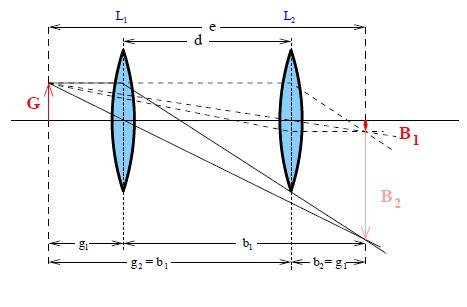
\includegraphics[width=0.6\linewidth]{../../Besselmethode}
	\caption{Bildkonstruktion des Linsensystems und Bestimmung der Brennweite nach der Bessel-Methode, \cite[4]{anleitung408}.}
	\label{fig:besselmethode}
\end{figure}
Weiterhin wird aus der Abbildung \ref{fig:besselmethode} folgendes abgelesen:
\begin{equation*}
e = g_1 + b_1 = g_2 + b_2
\end{equation*}
sowie
\begin{equation*}
d = g_1 - b_1 = g_2 - b_2.
\end{equation*}
Mit Hilfe der obigen Formeln lässt sich die Brennweite $f$ ausrechnen:
\begin{equation}
f = \frac{e^2-d^2}{4e}.
\end{equation}

\subsection{Bestimmung der Brennweite nach der Abbe-Methode}
\label{sec:Abbe}

Nach der Methode von Abbe(s. Abbildung \ref{fig:abbemethode}) wird die Brennweite $f$ eines Linsenssystems bestimmt. Mit Hilfe vom Abbildungsmaßstab $V$ wird die Brennweite und die Lage der Hauptebenen ermittelt. Damit die Gegenstandsweite $g'$ und die Bildweite $b'$ gemessen werden können, wird einen beliebigen Punkt $A$ ausgewählt. Für die Bildweite $b'$ und die Gegenstandsweite $g'$ ergeben sich die folgenden Formeln:
\begin{align}
g' &= g + h = f \cdot \left(1 + \frac{1}{V}\right) + h \\
b' &= b + h'= f \cdot (1 + V) + h'.
\end{align}

\begin{figure}[h!]
	\centering
	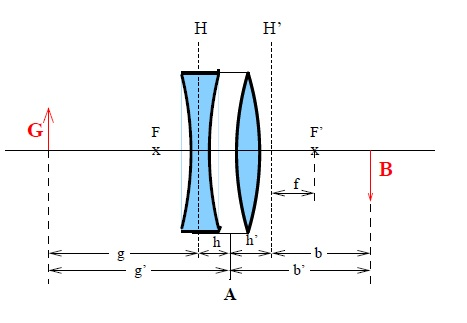
\includegraphics[width=0.6\linewidth]{../../Abbemethode}
	\caption{Bildkonstruktion des Linsensystems und Bestimmung der Brennweite nach der Abbe-Methode, \cite[5]{anleitung408}.}
	\label{fig:abbemethode}
\end{figure}
